\documentclass[11pt,a4paper]{article}

\usepackage[margin=2.2cm]{geometry}
\usepackage[T1]{fontenc}
\usepackage{lmodern}
\usepackage{amsmath,amssymb}
\usepackage{graphicx}
\usepackage{booktabs}
\usepackage{float}
\usepackage{caption}
\usepackage{enumitem}
\usepackage[hidelinks]{hyperref}
\usepackage{xcolor}
\usepackage{microtype}

\graphicspath{{../plots/}}
\setlist{itemsep=2pt,topsep=4pt}
\captionsetup{font=small}

\newcommand{\E}{\mathbb{E}}
\newcommand{\R}{\mathbb{R}}

\title{\textbf{Contextualizing Fairness:}\\ \textbf{Extending $p$-Mean Social Welfare to Linear Contextual Bandits}\\[4pt]
\large CS6106 Multi-Agent Machine Learning: Course Project Report, Team 04}
\author{Kunj Bhesaniya (23B0995) \and Dhruvraj Merchant (23B1041)\\[2pt]
\small Department of Computer Science and Engineering, IIT Bombay}
\date{November 2026}

\begin{document}
\maketitle

\begin{center}
\small Code: \url{https://github.com/KunjBhesaniya10/pmean-linear-bandits}
\end{center}

%=====================================================================
\section{Introduction}

In a normal multi-armed bandit the goal is to maximise total reward, i.e.\ minimise the average regret. When every round is a different person (a patient in a trial, a user getting a recommendation), this objective does not care who gets a bad round. An algorithm can give a few people very bad arms early on and still have small average regret.

$p$-mean social welfare fixes this by replacing the arithmetic mean of the per-round expected rewards with the power mean $M_p$. With $p=1$ we get back the usual utilitarian objective, $p=0$ gives the geometric mean (Nash social welfare), and $p\to-\infty$ only looks at the worst-off round (Rawlsian / egalitarian)~\cite{moulin2004}. So one parameter covers the whole range of fairness notions.

Our base paper is Sarkar, Pandey and Ray Chowdhury~\cite{sarkar2025}, \emph{``Revisiting Social Welfare in Bandits: UCB is (Nearly) All You Need''}. They show that a simple algorithm, Welfarist-UCB (uniform exploration with a data-adaptive stopping rule, then plain UCB), gets near-optimal $p$-mean regret for every $p$, with weaker assumptions than earlier work~\cite{barman2023,krishna2025}.

For linear bandits, fairness has been studied for Nash regret by LinNash~\cite{sawarni2023}, and for general $p$ by FairLinBandit~\cite{sarkar2026}. Both assume a \emph{fixed} arm set: their exploration uses a D-optimal design (and, in FairLinBandit, a John-ellipsoid distribution) computed over the whole arm set before learning starts. In most real uses like recommendation this is not the case. Each round a different user arrives with a different set of candidate items, so the arm set changes every round and there is nothing fixed to compute these objects over.

This is the setting of our project: \textbf{$p$-mean welfare in linear contextual bandits where the arm set is not fixed}. We did two things:
\begin{enumerate}
  \item \textbf{Reproduced} the Welfarist-UCB experiments (a)--(f) of the base paper from scratch.
  \item \textbf{Extended} the explore-then-UCB idea to the contextual setting. Since no geometry can be precomputed, we designed two data-adaptive versions of the exploration phase and stopping rule, and compared them on synthetic data and on MovieLens-1M.
\end{enumerate}
Our extension is empirical. We do not have a regret bound for it.

%=====================================================================
\section{Problem Setup}

\subsection{Multi-armed bandit with $p$-mean regret}
There are $k$ arms with unknown means $\mu_1,\dots,\mu_k\ge 0$ and $\sigma^2$-sub-Gaussian rewards. Let $\mu^\star=\max_i\mu_i$. At round $t=1,\dots,T$ the learner pulls $I_t$ using only past observations. The $p$-mean regret and Nash regret are
\[
R^p_T=\mu^\star-\Big(\frac1T\sum_{t=1}^T \E[\mu_{I_t}]^p\Big)^{1/p},\qquad
NR_T=\mu^\star-\Big(\prod_{t=1}^T \E[\mu_{I_t}]\Big)^{1/T}\quad(p=0).
\]
$R^p_T$ increases as $p$ decreases, so smaller $p$ is a harder (fairer) objective. For $p\le 0$ one round with expected reward close to zero can push the welfare towards zero, which is why plain UCB has no guarantee here.

\subsection{Linear contextual bandit}
In round $t$ a user $u_t$ arrives and is shown a candidate set $\mathcal{C}_t$ of $K$ items. The feature of item $i$ for user $u$ is $x=z_u\otimes y_i$ (Kronecker product of user and item features) and the expected reward is $\langle x,\theta^\star\rangle$ for an unknown $\theta^\star\in\R^d$. Since the best reward changes every round, we measure regret against the per-round optimum:
\[
R^p_T=M_p(r^\star_1,\dots,r^\star_T)-M_p(\E[r_1],\dots,\E[r_T]),\qquad r^\star_t=\max_{a\in\mathcal{C}_t}\langle x_a,\theta^\star\rangle .
\]
With one user and a fixed arm set this is the usual linear bandit $p$-mean regret. On MovieLens we also report a \textbf{normalised group utility} for each demographic group $g$: the sum of $\E[r_t]$ over rounds where a member of $g$ arrived, divided by the same sum for the optimal policy (1.0 is perfect). The group welfare is $M_{-2}$ of these 30 group utilities.

%=====================================================================
\section{Approach}

\subsection{Welfarist-UCB (base paper)}
\begin{itemize}
  \item \textbf{Phase I:} in every block of $k$ rounds pull the arms in a fresh random permutation. Each round has expected reward at least $\mu^\star/k$, so the welfare never collapses.
  \item \textbf{Stopping rule:} with $w_i=2\sqrt{2\sigma^2\log T/n_i}$, stop the first time some arm has $\hat\mu_i>w_i$ and $n_i>192\,p_a^2\sigma^2\log T/(\hat\mu_i-w_i)^2$, where $p_a=1$ for $p\ge-1$ and $p_a=p$ otherwise. Basically the best arm's LCB must be positive and large compared to its own width. For $p<-1$ exploration grows like $p^2$.
  \item \textbf{Phase II:} standard UCB with index $\hat\mu_i+w_i$.
\end{itemize}
Baselines from the paper: NCB~\cite{barman2023} for Nash regret and Explore-then-UCB~\cite{krishna2025}, which explores for a fixed $p$-dependent number of rounds.

\subsection{What changes when the arm set is not fixed}
In a fixed-arm linear bandit, one can compute a design over the arm set that covers every feature direction equally, and a distribution with a guaranteed reward floor. With contexts, $\mathcal{C}_t$ depends on the user and is new each round, so neither object exists in advance. Also, uniform sampling over candidates is no longer uniform over \emph{feature directions}: if only a few items or users use some coordinate, that direction is rarely seen. So the question is how Phase~I and the stopping rule should look when nothing can be precomputed.

\subsection{Adaptation 1: uniform transfer}
This is the most direct transfer of Welfarist-UCB.
\begin{itemize}
  \item \textbf{Phase I:} pick $a_t\sim\mathrm{Uniform}(\mathcal{C}_t)$.
  \item \textbf{Stopping:} with ridge estimate $\hat\theta_t$ and design matrix $V_t=\lambda I+\sum_s x_sx_s^\top$, stop as soon as some candidate satisfies
  \[
  \mathrm{LCB}(x_a)=\langle x_a,\hat\theta_t\rangle-\beta\|x_a\|_{V_t^{-1}}>0
  \quad\text{and}\quad
  \mathrm{LCB}(x_a)\ge\kappa\,|p_a|\,\beta\,\|x_a\|_{V_t^{-1}} .
  \]
  The width $\sqrt{1/n_i}$ simply becomes $\beta\|x_a\|_{V_t^{-1}}$. We use $\beta=\sigma\sqrt{2\log T}+\sqrt{\lambda}S$, the Abbasi-Yadkori radius~\cite{abbasi2011} without the $d\log t$ term, as most practical LinUCB code does (with that term nothing stops within our horizons).
  \item \textbf{Phase II:} LinUCB~\cite{li2010}, warm-started with $V_\tau$ and $\hat\theta_\tau$ from Phase~I.
\end{itemize}

\subsection{Adaptation 2: 50/50 uniform and greedy D-optimal exploration}
Same stopping rule and Phase~II; only Phase~I changes. In each exploration round, with probability $1/2$ we take a uniform candidate (to keep a reward floor as in Welfarist-UCB), and with probability $1/2$ we take
\[
a_t=\arg\max_{a\in\mathcal{C}_t}\|x_a\|_{V_t^{-1}},
\]
the candidate whose prediction we are least sure about. Adding this $x_a$ gives the largest increase of $\det V_t$, so it is a greedy one-step D-optimal design~\cite{lattimore2020} over whatever candidates are available right now, and it needs nothing precomputed. The intuition is that the most uncertain candidates are usually the ones in rare feature directions, so the algorithm learns those directions on purpose instead of waiting to hit them by chance.

The cost is that the max-width candidate can have low reward, so in easy instances where uniform sampling already covers everything, the extra steps are wasted rounds.

%=====================================================================
\section{Implementation}

Everything is written from scratch in Python (package \texttt{pmlb}), with the inner loops compiled by Numba (\texttt{@njit}), since experiment (a) alone is $50\times10^7$ rounds per algorithm.
\begin{itemize}
  \item \texttt{src/pmlb/welfare.py}: $p$-mean, running $p$-mean, $p$-mean regret curves, contextual regret and group utilities.
  \item \texttt{src/pmlb/mab/algorithms.py}: Welfarist-UCB, NCB and Explore-then-UCB. Constants follow the authors' public code (the stopping constant is $800\,p_a^2\sigma^2\log T$ in their code vs.\ 192 in the paper text).
  \item \texttt{src/pmlb/linear/algorithms.py}: the two adaptations and LinUCB. $V_t^{-1}$ is kept with $O(d^2)$ Sherman--Morrison updates instead of re-inverting. Widths skip zero coordinates, which matters for MovieLens where $x$ is sparse ($d=180$).
  \item \texttt{src/pmlb/linear/lin\_nash.py} and \texttt{fair\_lin\_bandit.py}: reference implementations of the fixed-arm methods LinNash~\cite{sawarni2023} and FairLinUCB~\cite{sarkar2026}.
  \item \texttt{src/pmlb/data/movielens.py}: builds the MovieLens bandit (below).
  \item \texttt{experiments/}: one script per set of results; \texttt{scripts/run\_all\_experiments.py} runs everything.
  \item \texttt{tests/}: 44 pytest tests ($p$-mean identities and monotonicity in $p$, Sherman--Morrison against direct inversion, kernels only pick real candidates and are reproducible under a seed, exploration grows as $p$ decreases, MovieLens group encoding). All pass in about 20\,s.
\end{itemize}
All runs are seeded, and rerunning gives exactly the same numbers.

\paragraph{MovieLens-1M environment.} We use MovieLens-1M~\cite{harper2015}. Reward is ``user likes the movie'' (rating $\ge 4$), a Bernoulli reward. User features $z$ (30-dim) are one-hot gender (2), age band (7) and occupation (21), so every demographic group has its own coordinates and small groups (e.g.\ 17 farmers, 0.3\% of rounds) are rare feature directions. Item features $y$ (6-dim) are a bias, the movie's like rate, and a rank-4 SVD embedding of the centred like matrix. $\theta^\star$ (180-dim) is the ridge fit of like $\sim z_u\otimes y_i$ over all ratings of the 300 most-rated movies, so the environment is exactly linear and its expected rewards are the fitted like probabilities (all inside $(0,1)$; the code checks this). Each round a uniformly random user arrives with 20 random candidate movies; $T=50{,}000$, 20 runs.

%=====================================================================
\section{Results}

\subsection{Reproduction of Welfarist-UCB ($k=50$, 50 runs each)}
Instances are drawn exactly as in the authors' code (\texttt{np.random.seed(42)}), so the arm means are the same as theirs.

\begin{table}[H]
\centering\small
\begin{tabular}{llllr}
\toprule
Expt & Setting & Algorithm & Regret at $T$ & Phase I length $\tau$\\
\midrule
(a) & Bernoulli, $p=0$, $T=10^7$ & NCB & 0.225 & 3{,}349{,}088\\
    & & \textbf{Welfarist-UCB} & \textbf{0.062} & 828{,}816\\
(b) & Gaussian $\sigma=20$, $p=0$, $T=10^6$ & NCB & 1.75 & 2{,}487\\
    & & \textbf{Welfarist-UCB} & \textbf{0.182} & 266\\
(c) & Gaussian, $p=0.5$ & Explore-then-UCB & 45.3 & 79{,}955\\
    & & \textbf{Welfarist-UCB} & \textbf{0.16} & 266\\
(d) & Gaussian, $p=-0.5$ & Explore-then-UCB & 18.1 & 22{,}365\\
    & & \textbf{Welfarist-UCB} & \textbf{0.22} & 266\\
(e) & Gaussian, $p=-1.5$ & Explore-then-UCB & 3.85 & 3{,}163\\
    & & \textbf{Welfarist-UCB} & \textbf{0.72} & 592\\
\bottomrule
\end{tabular}
\caption{Reproduction of experiments (a)--(e).}
\end{table}

\begin{figure}[H]
\centering
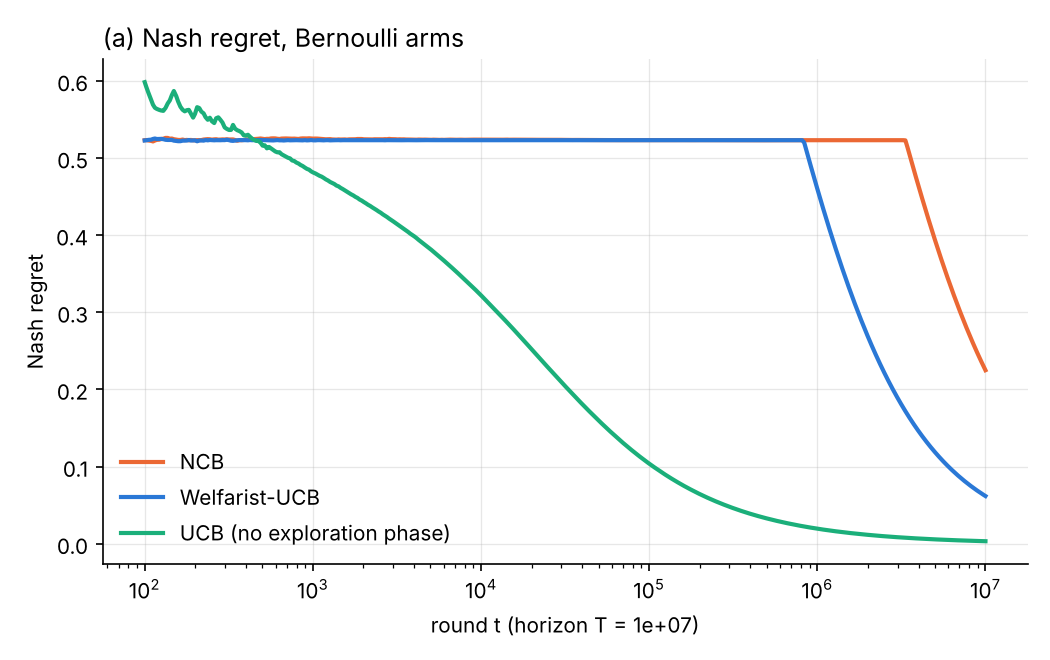
\includegraphics[width=0.62\linewidth]{mab_reproduction/expt_a.png}
\caption{Experiment (a): Nash regret of Welfarist-UCB vs.\ NCB on Bernoulli arms.}
\end{figure}

Our numbers match the paper's figures: Welfarist-UCB beats NCB by about $4\times$ in (a) and $10\times$ in (b), and beats Explore-then-UCB at all three $p$, by two orders of magnitude for $p\ge-0.5$. The gap gets smaller at $p=-1.5$ because the stopping rule now has $p_a^2=2.25$ and explores longer.

\paragraph{Effect of $p$ (experiment f).}
\begin{table}[H]
\centering\small
\begin{tabular}{lccccc}
\toprule
$p$ & 1 & 0 & $-1$ & $-2$ & $-5$\\
\midrule
Regret at $T$ & 0.13 & 0.17 & 0.24 & 1.29 & 27.0\\
$\tau$ & 276 & 273 & 275 & 1{,}010 & 5{,}922\\
\bottomrule
\end{tabular}
\caption{Welfarist-UCB across $p$ (Gaussian arms, $T=10^6$).}
\end{table}
For $p\ge-1$ the stopping rule does not depend on $p$, so $\tau$ is basically constant. Below $-1$ it scales with $p^2$ ($3.7\times$ at $p=-2$, $21\times$ at $p=-5$), which is the ``no free fairness'' cost the paper predicts.

\begin{figure}[H]
\centering
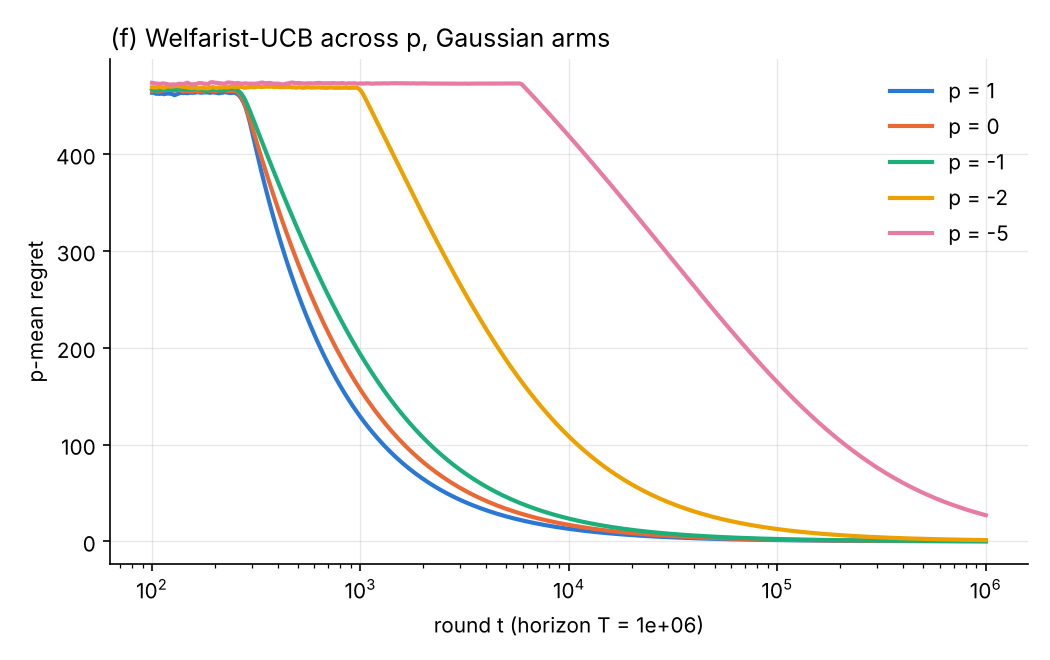
\includegraphics[width=0.62\linewidth]{mab_reproduction/expt_f.png}
\caption{Experiment (f): Welfarist-UCB regret for different $p$.}
\end{figure}

\subsection{Synthetic linear experiments (Nash regret, $p=0$, $\kappa=10$, 15 runs)}

\paragraph{Experiment 1: benign arms} ($d=6$, $K=50$, $T=50{,}000$). Features and $\theta^\star$ are positive and random, so every direction is common; means lie in $[0.65,0.96]$.

\begin{table}[H]
\centering\small
\begin{tabular}{lrcc}
\toprule
 & $\tau$ & Nash regret at $t=10^4$ & Nash regret at $T$\\
\midrule
Adaptation 1 (uniform) & 2{,}661 & 0.045 & \textbf{0.0146}\\
Adaptation 2 (50/50 D-opt) & 2{,}812 & 0.057 & 0.0169\\
\bottomrule
\end{tabular}
\end{table}

Both stop early and the regret goes to near zero after the switch to LinUCB. Adaptation~1 is slightly better here. This is what we expected: when all directions are already covered by uniform sampling, the max-width steps just pick lower-reward arms during Phase~I, which shows up as the higher plateau of Adaptation~2 before $\tau$.

\begin{figure}[H]
\centering
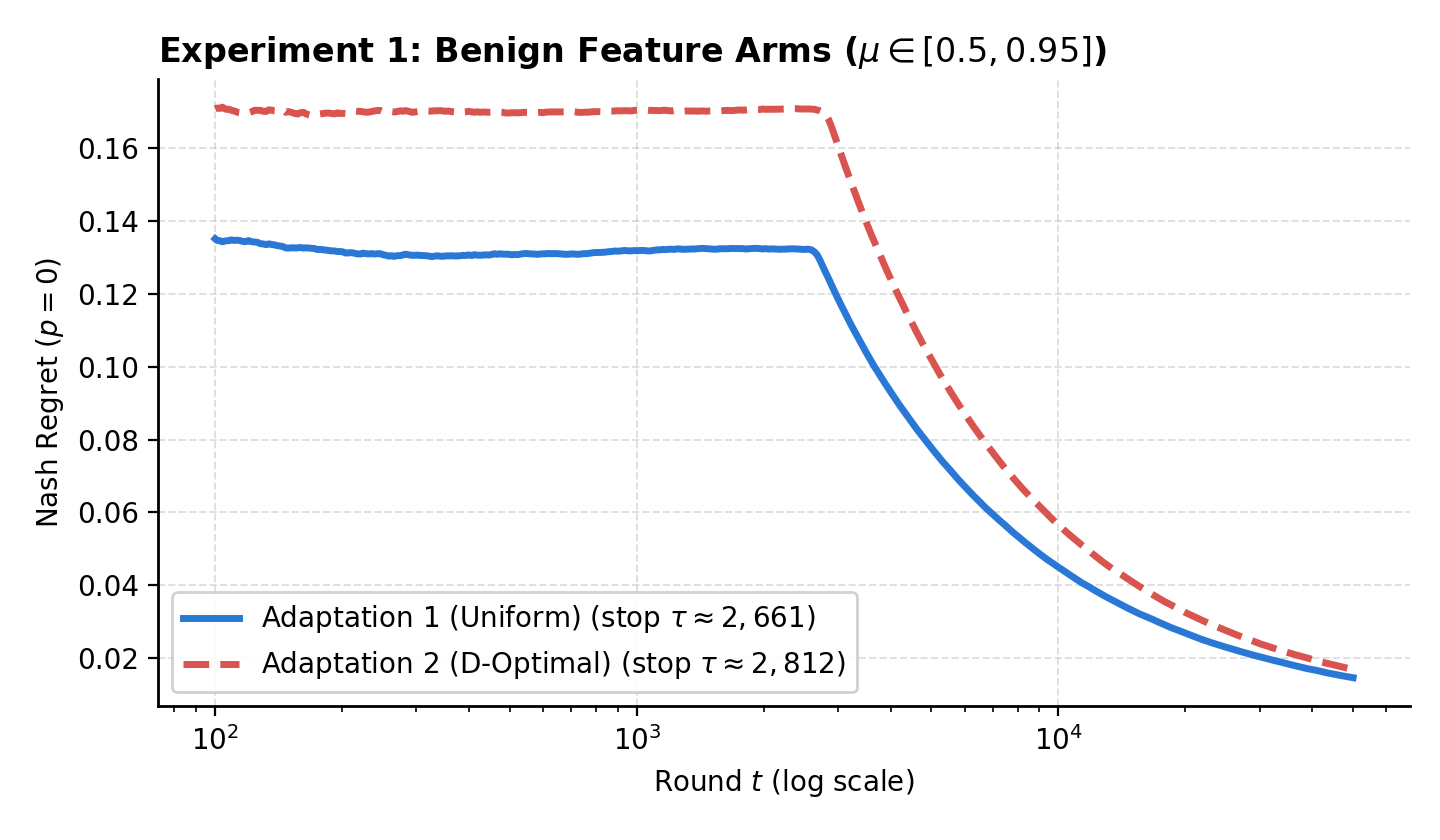
\includegraphics[width=0.62\linewidth]{linear_synthetic/expt1_variant1_wins.png}
\caption{Experiment 1: benign feature arms.}
\end{figure}

\paragraph{Experiment 2: rare direction} ($d=6$, $K=100$, $T=30{,}000$). 98 ``common'' arms use only the first four coordinates and have mediocre means (0.21 to 0.33). Only two arms have weight on the fifth coordinate, and the optimum (0.95) is one of them.

\begin{table}[H]
\centering\small
\begin{tabular}{lrcc}
\toprule
 & $\tau$ & Nash regret at $t=10^4$ & Nash regret at $T$\\
\midrule
Adaptation 1 (uniform) & 15{,}478 & 0.645 & 0.419\\
Adaptation 2 (50/50 D-opt) & \textbf{10{,}973} & \textbf{0.526} & \textbf{0.242}\\
\bottomrule
\end{tabular}
\end{table}

Here Adaptation~2 has about $1.7\times$ lower final regret and stops about 4{,}500 rounds earlier. With uniform sampling the rare direction is seen in only 2 of every 100 pulls, so no arm becomes certified for a long time (the common arms are too low for the LCB condition with $\kappa=10$). The max-width steps go straight to the rare direction, so the optimum's LCB grows faster and the rule fires earlier.

\begin{figure}[H]
\centering
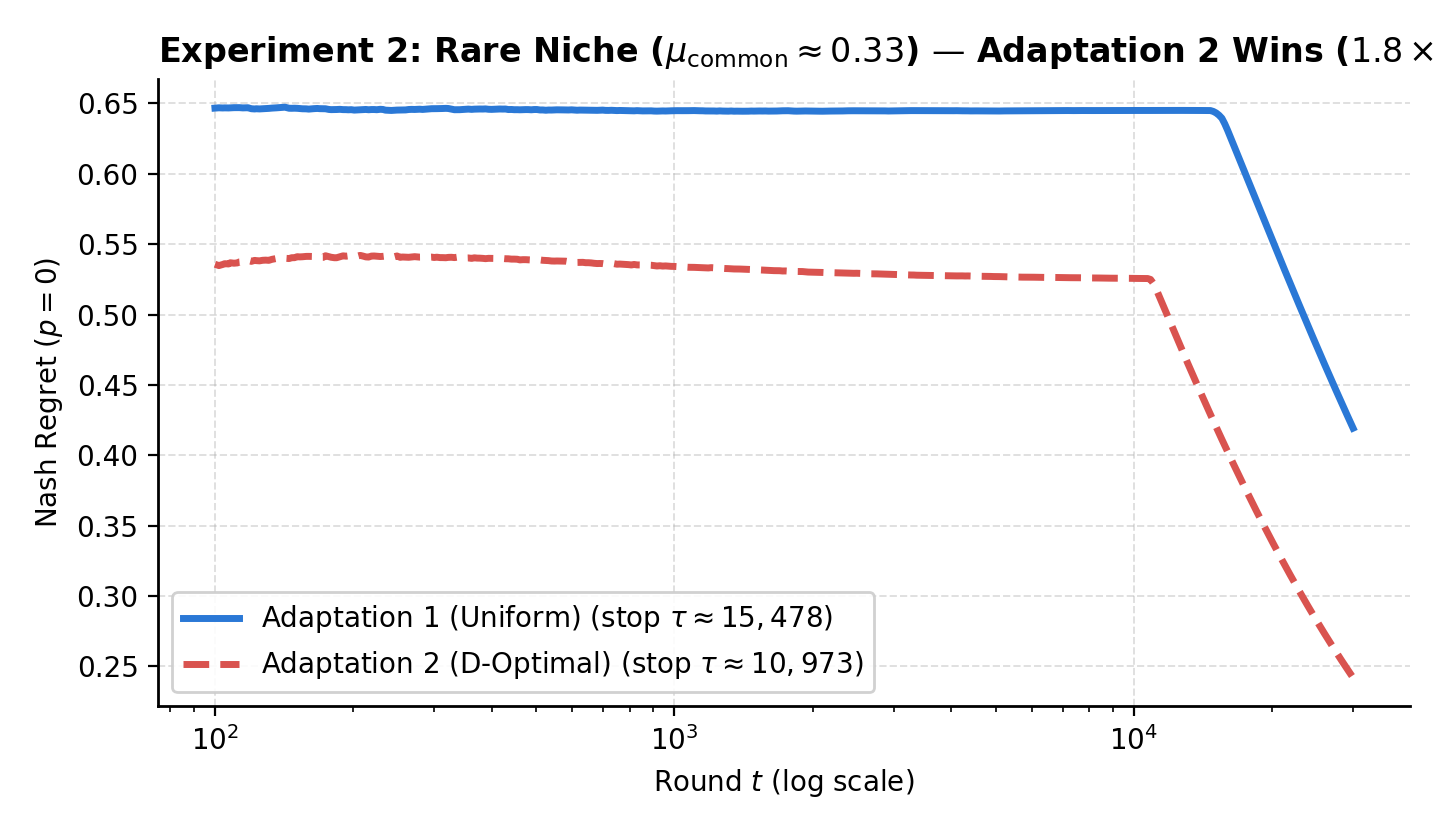
\includegraphics[width=0.62\linewidth]{linear_synthetic/expt2_variant2_wins.png}
\caption{Experiment 2: rare niche features.}
\end{figure}

\subsection{MovieLens-1M ($d=180$, $K=20$, $T=50{,}000$, $\kappa=1$, 20 runs)}
With $\kappa=10$ the stopping rule did not fire within 50{,}000 rounds on MovieLens ($d=180$ is much larger than the synthetic $d=6$), so here we use $\kappa=1$.

\begin{table}[H]
\centering\small
\setlength{\tabcolsep}{4pt}
\begin{tabular}{lcrccccc}
\toprule
 & $p$ in rule & $\tau$ & Agg.\ utility & Regret $p{=}1$ & Regret $p{=}0$ & Regret $p{=}{-2}$ & Group $M_{-2}$\\
\midrule
Adaptation 1 & 0 & 1{,}205 & 0.9494 & 0.0447 & 0.0489 & 0.0650 & 0.9353\\
Adaptation 2 & 0 & 1{,}251 & 0.9500 & 0.0442 & 0.0485 & 0.0633 & 0.9358\\
Adaptation 1 & $-2$ & 2{,}708 & 0.9451 & 0.0485 & 0.0527 & 0.0654 & 0.9318\\
Adaptation 2 & $-2$ & 2{,}681 & 0.9465 & 0.0473 & 0.0521 & 0.0674 & 0.9329\\
\bottomrule
\end{tabular}
\caption{MovieLens-1M results.}
\end{table}

\begin{figure}[H]
\centering
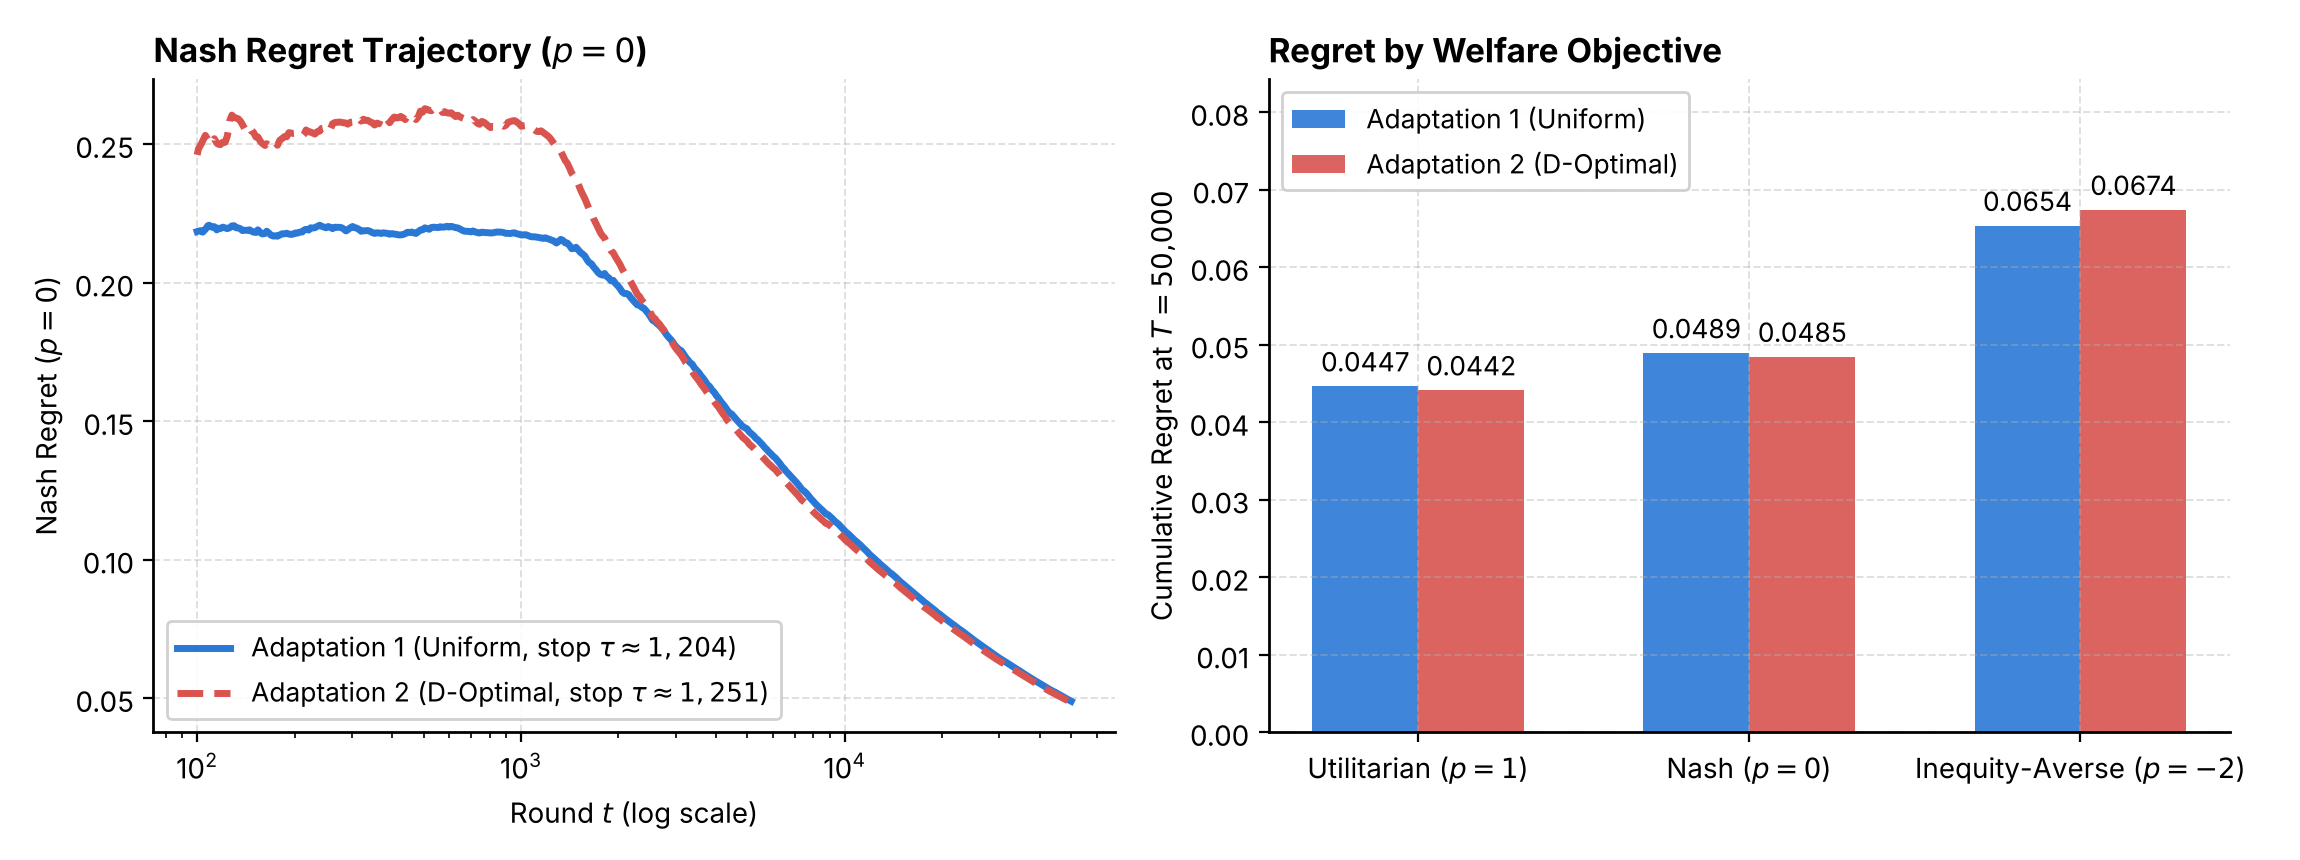
\includegraphics[width=\linewidth]{movielens/movielens_clean.png}
\caption{MovieLens: Nash regret over time (left) and final $p$-mean regret (right; the $p=-2$ bars use the run with $p=-2$ in the stopping rule).}
\end{figure}

Both adaptations leave Phase~I after a little over 1{,}000 rounds and then behave almost the same under LinUCB. Adaptation~2 is slightly better on most numbers when run with $p=0$, and slightly worse on the $p=-2$ regret when run with $p=-2$. These differences are in the third decimal and we did not run significance tests, so we read this as roughly a tie.

\paragraph{Groups.} The smallest group, farmers (0.33\% of rounds, about 165 rounds per run), gets 0.862 with Adaptation~2 vs.\ 0.855 with Adaptation~1, and is the worst-off group under both. Across all 30 groups, Adaptation~2 is higher on 18 and lower on 12, so it is not a uniform improvement. The worst-off groups for both are small occupations (farmer, unemployed, homemaker, tradesman) and older users, i.e.\ exactly the rare feature directions.

\begin{figure}[H]
\centering
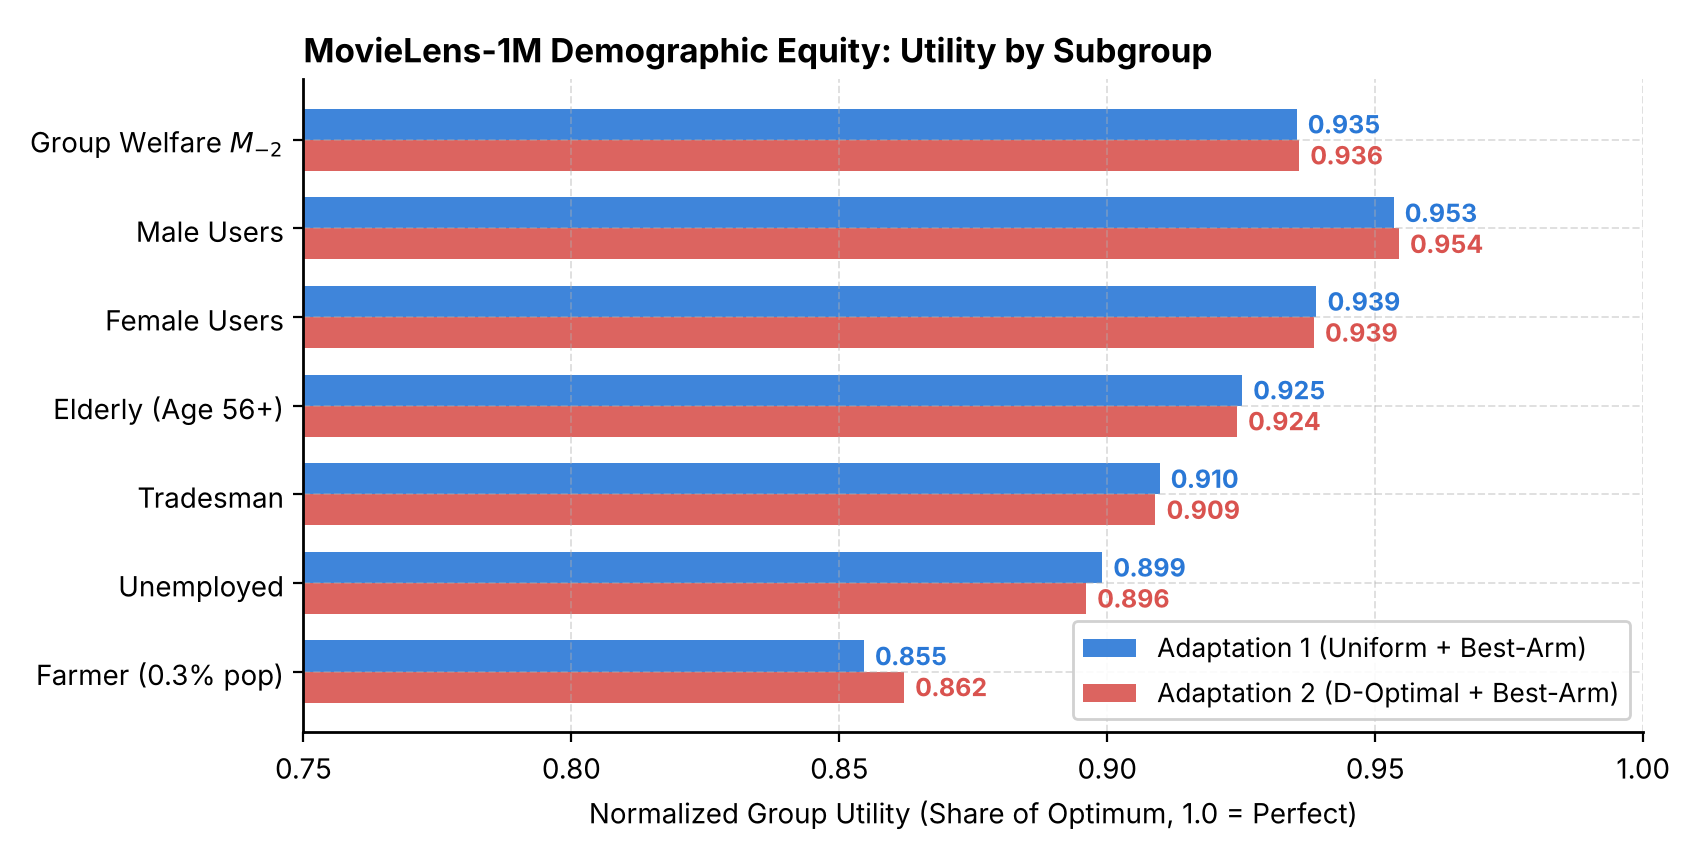
\includegraphics[width=0.78\linewidth]{movielens/movielens_demographics.png}
\caption{MovieLens: normalised utility for selected demographic groups.}
\end{figure}

\subsection{Summary}
\begin{itemize}
  \item The reproduction works and matches the paper.
  \item In the contextual setting, a direct transfer of Welfarist-UCB (Adaptation~1) is already fine when every feature direction is common; the greedy D-optimal steps (Adaptation~2) cost a little there.
  \item When the good arm lies in a rare direction, Adaptation~2 learns it faster and gets about $1.7\times$ lower Nash regret.
  \item On MovieLens both are almost tied; the smallest groups are the worst-off under both.
\end{itemize}

%=====================================================================
\section{Challenges and Learnings}

\subsection{Challenges}
\begin{itemize}
  \item \textbf{No fixed geometry to work with.} The fixed-arm tools (a D-optimal design or a reward-floor distribution over the arm set) cannot be computed when the candidate set is new every round. We had to find exploration rules that only use the current candidates and the data seen so far, which led to the greedy max-width step in Adaptation~2.
  \item \textbf{Stopping constant does not carry over across dimensions.} $\kappa=10$ works for $d=6$ but never stops within 50{,}000 rounds on MovieLens ($d=180$). We had to use $\kappa=1$ there, which is a tuning choice we cannot justify theoretically. Similarly, the full Abbasi-Yadkori radius made every method explore for the whole horizon, so we dropped its $d\log t$ term.
  \item \textbf{Matching the paper's constants.} The stopping constant in the paper text (192) differs from the authors' code (800). Since we were reproducing their figures, we followed the code.
  \item \textbf{Compute.} Experiment (a) is $10^7$ rounds $\times$ 50 runs per algorithm. Plain Python was far too slow, so all kernels are compiled with Numba, and the linear kernels use Sherman--Morrison updates and sparse width computation.
  \item \textbf{Data access.} The official MovieLens site was unreachable for us, so the download script falls back to a GitHub mirror and checks the size of the data (1{,}000{,}209 ratings, 6{,}040 users) before using it.
\end{itemize}

\subsection{Learnings}
\begin{itemize}
  \item Exploring for rare directions is not free. The 50/50 change helps only when some direction is actually rare, and costs a little on easy instances. We think this trade-off is the honest result rather than a clear winner.
  \item Fairness has a price in exploration: in the reproduction, $\tau$ grows with $p^2$ for $p<-1$, and regret grows with it.
  \item In the contextual setting, the worst-off groups are the small ones, because their feature directions are seen least. Per-round $p$-mean welfare and fairness across groups are related but not the same thing.
  \item A regret bound for $p$-mean welfare in contextual linear bandits with arbitrary changing candidate sets is still open as far as we know.
\end{itemize}

%=====================================================================
\section{Team Contributions}
\textcolor{red}{[To be filled in by the team.]}

%=====================================================================
\begin{thebibliography}{10}\small
\bibitem{sarkar2025} D.~Sarkar, N.~Pandey, S.~Ray Chowdhury. Revisiting Social Welfare in Bandits: UCB is (Nearly) All You Need. arXiv:2510.21312, 2025.
\bibitem{sarkar2026} D.~Sarkar, N.~Pandey, S.~Ray Chowdhury. Improved Algorithms for Nash Welfare in Linear Bandits. ICML 2026, arXiv:2601.22969.
\bibitem{barman2023} S.~Barman, A.~Khan, A.~Maiti, A.~Sawarni. Fairness and Welfare Quantification for Regret in Multi-Armed Bandits. AAAI 2023.
\bibitem{krishna2025} A.~Krishna, P.~G.~John, A.~Barik, V.~Y.~F.~Tan. $p$-Mean Regret for Stochastic Bandits. AAAI 2025.
\bibitem{sawarni2023} A.~Sawarni, S.~Pal, S.~Barman. Nash Regret Guarantees for Linear Bandits. NeurIPS 2023.
\bibitem{abbasi2011} Y.~Abbasi-Yadkori, D.~P\'al, Cs.~Szepesv\'ari. Improved Algorithms for Linear Stochastic Bandits. NeurIPS 2011.
\bibitem{li2010} L.~Li, W.~Chu, J.~Langford, R.~E.~Schapire. A Contextual-Bandit Approach to Personalized News Article Recommendation. WWW 2010.
\bibitem{lattimore2020} T.~Lattimore, Cs.~Szepesv\'ari. \emph{Bandit Algorithms}. Cambridge University Press, 2020.
\bibitem{moulin2004} H.~Moulin. \emph{Fair Division and Collective Welfare}. MIT Press, 2004.
\bibitem{harper2015} F.~M.~Harper, J.~A.~Konstan. The MovieLens Datasets: History and Context. ACM TiiS, 2015.
\end{thebibliography}

\end{document}
